%Preambule met standaardinstellingen
\documentclass[a4paper,oneside]{report}
%Noot: zorg ervoor dat Nederlandse woordsplitsing geactiveerd is.
\usepackage[dutch]{babel}
% Noot: je kan het graphicxpakket een optie dvips of pdftex doorgeven
% in dat geval oet je ze ook aan iiiscriptie doorgeven, dus bijvoorbeeld
% \usepackage[dvips]{graphicx}
% \usepackage[dvips]{iiiscriptie}
\usepackage{graphicx}
\usepackage{iiiscriptie}
%Nuttig pakket voor URL's
\usepackage{url}
\def\latex{$\mathrm{L\!\!^{{}_{\scriptstyle A}} \!\!\!\!\!\;\; T\!_{\displaystyle E} \!
X}$}
%
%Invullen velden voor titelpagina.
%
\departement{Departement Toegepaste Ingenieurswetenschappen}
\deptadres{Schoonmeersstraat 52 - 9000 Gent}
\studiejaar{3e Bachelor Informatica}
\soortrapport{
Visualisatie van xkcd
}
\title{Richtlijnen voor projectverslagen}
\author{
\begin{tabular}{ll}
Groep 6 & Jan Acke\\
&Davy Loose\\
&Simon Gaeremynck\\
&Christian Vuerings\\
\end{tabular}
}
\begin{document}
\maketitle
\pagenumbering{roman}
\tableofcontents
\addcontentsline{toc}{chapter}{Inhoudsopgave}
\pagenumbering{arabic}
\chapter{Inleiding}
Het netwerkvisualisatieproject is een project van 4 studenten voor het vak systeemanalyse en ontwerp. De bedoeling van het project is om een simulatie van een computernetwerk na te bootsen. Elke computer in het netwerk kan bestanden versturen naar zijn direct verbonden buren want het netwerk is opgebouwd als een p2p netwerk. Zo een bestand kan zowel goedaardig als kwaadaardig zijn. De goedaardige bestanden, aangeduid in de simulatie als groene sterren, doen niets met de computer. Men kan dit zien als gewoon mailverkeer. De slechte bestanden kunnen we zien als mailverkeer met een virus attachment. Hierdoor kan de computer besmet worden met een virus, trojan of worm. Hierna zal de besmette pc ook dit virus beginnen doorsturen naar zijn directe buren. Zo kan men via de simulatie zien hoe een virus zich kan verspreiden in een computernetwerk.\\*
Het belangrijkste onderdeel van dit project was het opbouwen van een deftig ontwerp voor het cre�ren van de software. Hierdoor moesten we gebruik maken van technieken die we gezien hebben in de les. Eenmaal het ontwerp klaar was konden we beginnen aan het programmeren van de simulatie. Natuurlijk moest het vooraf opgemaakte ontwerp gevolgd worden. De keuze van programmeertaal mochten we zelf kiezen. Wij kozen voor een combinatie van HTML5 en Javascript. Dit komt ons goed uit omdat het project moet kunnen draaien op een standaard pc van school, hierdoor waren we besturingssysteem onafhankelijk.


\chapter{Model}
\section{Statisch model}
\subsection{Klassenmodel}
We beschrijven voor iedere klasse wat hij precies doet.
\lemma{Bestand}: Dit is het object die wordt doorgestuurd tussen de verschillende computers. Het bestand kan opgesplitst worden in 2 sub onderverdelingen.
\lemma{GoedBestand}: Dit is een bestand die geef nare gevolgen heeft voor de computer die het ontvangt, men kan dit vergelijken met een email met alleen tekst.
\lemma{SlechtBestand}: Dit is een bestand die een virus, trojan of worm bevat. Via de gegevens  van het bestand kunnen we zo het risico berekenen dat de computer besmet wordt.
\lemma{Computer}: Zoals men kan verwachten is dit een object die bestanden kan ontvangen en versturen. Het is altijd verbonden met tenminste één andere computer. Aan de hand van een lijst van virussen dat de computer bevat kan hij virussen doorsturen naar buurcomputers.
\lemma{Beheersysteem}: Dit is het object die het scherm beïnvloed. Deze zorgt voor de demo modus van het systeem. Het beheersysteem zal de keuze maken welke computers er nieuwe buren krijgen, welke computers bestanden versturen en gekuist worden van virussen, en welke computers verwijderd zullen worden.
\lemma{VisualisatieBibliotheek}: Dit is een bibliotheek dat we gebruiken voor het tekenen van de graaf. Via deze bibliotheek kunnen we gemakkelijk zien welke computers er met elkaar verbonden zijn en kunnen we dit ook tekenen.

\eindlemma
\diagram{klassen_diagram}{Het klassendiagram}
\newpage
\diagram{crc_kaarten}{De CRC kaarten}
\newpage
\section{Dynamisch model}
We geven hieronder een lijst van alle taken.

\begin{figure}[h!]
\begin{center}

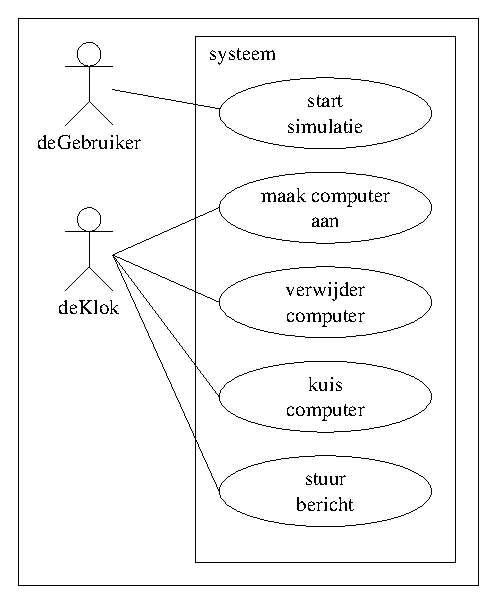
\includegraphics[scale=0.75]{taken_diagram2}

\caption{Takendiagram}
\end{center}
\end{figure}


\subsection{Start simulatie}
\lemma{Actor}
deGebruiker.

\lemma{Beschrijving}
Via deze taak kan de gebruiker de demo mode activeren en zal het beheersysteem op basis van de klok de verschillende taken automatisch uitvoeren.

\lemma{Sequentiediagram}
\diagram{seq_start_simulatie}{Start simulatie}

\newpage
\subsection{Maak computer aan}
\lemma{Actor}deKlok.

\lemma{Beschrijving}
De klok stuurt een bericht naar het BeheerSysteem dat er een computer mag aangemaakt worden. Er moet niet gewacht worden op een antwoord van de computer om verder te doen met het systeem. De computer zal wel een asynchroon antwoord sturen indien hij aangemaakt is.

\lemma{Sequentiediagram}
\diagram{seq_maak_computer_aan}{Maak computer aan}

\newpage
\subsection{Verwijder computer}
\lemma{Actor}deKlok.

\lemma{Beschrijving}
De klok stuurt een signaal naar het BeheerSysteem dat er een computer verwijderd mag worden. Het beheersysteem maakt dan een keuze uit alle computers en beslist welke computer er verwijderd mag worden. Hij stuurt dan een bericht naar deze computer, deze computer zal dan een antwoord terugsturen naar het beheersysteem dat deze verwijderd zal worden, zodat we deze ook uit de lijst van computers kunnen halen.

\lemma{Sequentiediagram}
\diagram{seq_verwijder_computer}{Verwijder computer}

\newpage
\subsection{Kuis computer}
\lemma{Actor}
deKlok.

\lemma{Beschrijving}
De klok stuurt een bericht naar het BeheerSysteem dat er computer mag gekuist worden, dit wil zeggen alle virussen verwijderen. Het beheersysteem zal dan willekeurig een computer kiezen, die hij kan kiezen uit de visualisatiebibliotheek, en een bericht sturen naar deze computer dat de virussen mogen verwijderd worden en zijn status van ‘IsBesmet’ op false mag zetten.

\lemma{Sequentiediagram}
\diagram{seq_kuis_computer}{Kuis computer}

\newpage
\subsection{Stuur bericht}
\lemma{Actor}
deKlok.

\lemma{Beschrijving}
De klok stuurt een bericht naar het beheersysteem dat er bestanden mogen doorgestuurd worden van een computer naar andere computers. Het beheersysteem roept de methode stuurBestand op van een willekeurig geselecteerde computer, deze zal dan een keuze maken welk soort bestand er verstuurd zal worden, dit kan een goed bestand zijn of een slecht bestand. Hierna roept de computer van al zijn buren de methode ontvangbestand op en stuurt dit bestand dan door. Dit alles gebeurt asynchroon zodat de computer niet hoeft te wachten op een antwoord van de te ontvangen computer.

\lemma{Sequentiediagram}
\diagram{seq_stuur_bericht}{Stuur bericht}

\newpage
\section{Woordenboek}
\subsection{Beheersysteem}
\lemma{leesConfig()} Leest het config bestand, config.js in en construeert de nodige objecten.
\lemma{startDemo()} De demo mode van het programma wordt nu gestart. Dit wil zeggen dat vanaf nu er automatisch computers aangemaakt zullen worden, virussen verspreid zullen worden, computers schoongemaakt kunnen worden en ook computers kunnen verwijderd worden.
\lemma{kuisComputer()} Het beheersysteem zal willekeurig een computer kiezen uit de lijst van aangemaakte computers en zal er 1 van verwijderen. Bij het verwijderen legt het beheersysteem de verbindingen tussen de buurcomputers. Om dit te realiseren zal het beheersysteem gebruik maken van de volgende lidfuncties:
\begin{itemize}
    \item Computer:verwijderVirussen()
\end{itemize}
\lemma{maakComputerAan()} Zoals gezegd zal deze functie een nieuwe computer aanmaken en zelf beslissen met wie hij verbonden zal worden.
\lemma{stuurBericht()} Het beheersysteem zal beslissen uit de lijst van computers welke computers er een bestand mogen sturen naar hun buren. Deze functie maakt gebruik van de volgende lidfuncties:
\begin{itemize}
    \item Computer:stuurBestand()
\end{itemize}
\lemma{verwijderComputer()} Het beheersysteem zal willekeurig een computer kiezen uit de lijst welke computer er verwijderd zal worden. Hiervoor maakt hij gebruik van de volgende lidfuncties:
\begin{itemize}
    \item Computer:geefVerbondenComputers()
    \item Computer:kanVerwijderdworden()
\end{itemize}
\subsection{Computer}
\lemma{kanVerwijderdWorden()} Deze methode geeft terug of de computer kan verwijderd worden. Dit wordt bepaald door zijn staat ‘isInternet’. Dit wil zeggen dat deze computer een lijst bevat met alle virussen en zodoende niet kan verwijderd worden indien we willen dat alle virussen nog doorgegeven kunnen worden.
\lemma{ontvangBestand(Bestand)} Het beheersysteem zal willekeurig een computer kiezen uit de lijst welke computer er verwijderd zal worden. Hiervoor maakt hij gebruik van de volgende lidfuncties:
\begin{itemize}
    \item Bestand:geefVerspreidingssnelheid()
    \item Bestand:geefType()
    \item Bestand:geefNaam()
\end{itemize}
\lemma{stuurBestand(Computer)} Via deze methode wordt een buur gekozen uit de lijst van verbonden computers. Naar deze computer zullen we dan een bestand sturen die bijvoorbeeld een virus kan bevatten.
\lemma{verwijderBestanden()} Hierin wordt de computer gekuist van alle virussen die hij heeft en wordt de staat ‘isBesmet’ op false gezet.
\lemma{geefVerbondenComputers()} Via deze methode kunnen we een lijst verbonden buren van de computer terugkrijgen.
\subsection{Bestand}
\lemma{geefVerspreidingsSnelheid()} Hierin kunnen we de verspreidingssnelheid van een virus terugkrijgen.
\lemma{geefType()} Via deze methode krijgen we het type bestand terug.
\lemma{geefNaam()} Zoals de methode al zegt krijgen we hier de naam van het bestand terug.
\subsection{VisualisatieBibliotheek}
\lemma{forceDirected()} De Visualisatie bibliotheek ondersteunt meerdere types van grafieken. Degene die hier gebruikt moet worden is het “ForceDirected” type.
\lemma{loadJSON()} Laad de config in met de data van het netwerk. Dit moet in het correcte formaat zijn.
\lemma{compute()} Zal de posities van de computers berekenen en de verbindingen ertussen. Dit levert telkens andere posities op. Dit mag enkel in het begin van de simulatie gebruikt worden.
\lemma{computeIncremental()} Voert de bovenstaande functie uit, maar in zo een manier dat de resources optimaal gebruikt worden.
\lemma{plot()} Tekent de berekende posities van de computers. Als er iets hertekent moet worden, zal deze functie gebruikt moeten worden.
\eindlemma

\newpage
\section{Aanvullingen}
%Deze paragraaf is optioneel, en kan gebruikt worden om elementen van het model in
%onder te brengen die niet bij elk project voorkomen, zoals
\begin{itemize}
\item Functioneel model
Ons functioneel model omschrijft de manier waarop een computer een bestand verstuurd. In eerste instantie wordt er gekozen of 
er een goed of een slecht bericht gestuurd wordt (Besmette computers kunnen nog steeds goede bestanden doorsturen). Als een goed
bestand wordt gekozen dan zal dit direct teruggegeven worden. Als er echter een slecht bestand gekozen wordt zal de computer aan de 
hand van het slechte bestand zijn verspreidingssnelheid bepalen welk slecht bestand doorgestuurd wordt. De kans om een bestand met 
lage verspreidingssnelheid door te sturen is lager dan de kans om een bestand met hoge verspreidingssnelheid door te sturen.

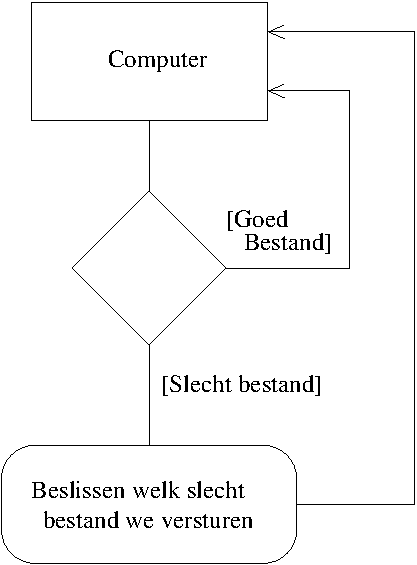
\includegraphics{funcmodel}
%\item Statendiagrammen.
%\item Databankontwerp in de vorm van EPR-diagrammen, tabeldefinities en dergelijke.
\end{itemize}
% In deze paragraaf worden ook bijkomende technische elementen vermeld. Zo dient
% bijvoorbeeld, bij het gebruik van het MVC-paradigma, hier vermeld worden welke elementen
% de view en de controller uitmaken.


\chapter{Realisatie}
\section{Hergebruik}
Er wordt veelvuldig gebruik gemaakt van een aantal publieke bibliotheken die op het eerste
zicht niet zo gemakkelijk zijn. Hieronder vind u een overzicht van deze bibliotheken en nog
extra informatie die handig is voor het volledig opbouwen van de simulatie.
\subsection{Force-Directed Graphs}
Het network dat moet opgebouwd worden is eigenlijk een graaf. Meer specifiek het is een
``Force-Directed'' of ``Force-Based'' graph \cite{ForceBasedGraph}.
Dit houdt in dat al de ``edges'', verbindingen tussen de computers, van min of meer gelijke afstand zijn.
\subsection{JavaScript InfoVis Toolkit}
De JavaScript InfoVis Toolkit \cite{InfoVis}, kortweg JIT, is een bibliotheek dat geschreven is voor interactieve
data visualizaties. Deze is in staat om een heel arsenaal grafen en grafieken te renderen, waaronder
de Force-Directed graaf.
De naam geeft het al weg, deze is geschreven in JavaScript en werkt met het html5 canvas object.
Het staat iedereen vrij deze bibliotheek te gebruiken aangezien ze beschikbaar gemaakt wordt onder
de Berkeley Software Distribution licensie.
Hoewel er onder veel developers smalend wordt gepraat over JavaScript, is de taal uitermate geschikt voor visualisaties
en laat ze perfect toe om ``object georienteerd'' te werken.
\subsection{GIT}
Om een optimale collaboratie te verkrijgen, gebruiken we GIT.
GIT laat toe om meerdere mensen samen op dezelfde source code te werken.
Op deze manier beschikt iedereen altijd over de laatste versies.

\section{Gebruik}
Het volstaat om het index.html bestand te openen in een moderne browser. De simulatie start van zodra de pagina is ingeladen.
Mocht de simulatie om één of andere reden falen, kan deze opnieuw gestart worden door de pagina te herladen.
\section{installatie}
Als u over een moderne browser beschikt hoeft er eigenlijk niets extra geinstalleerd worden.
Echter, voor een vlotte gebruikerservaring raden we aan om een van de volgende browsers te gebruiken.
\begin{itemize}
\item Chrome 8.0 of later. Er is een installer bijgevoegd op de CD-ROM.
\item Firefox 4 beta of later.
\end{itemize}


\chapter{Logboek}
Hieronder vind je een lijst met wie wat juist gedaan heeft op welk moment.
\begin{studentlog}{Jan Acke}
\logingang{26/11/10}{16}{45}{17}{45}
{Eerste labo}
\logingang{01/12/10}{08}{15}{10}{15}
{Tweede bijeenkomst - sequentiediagrammen aanmaken, takendiagram aanpassen en overlopen van geschikte software}
\logingang{03/12/10}{15}{45}{17}{15}
{Tweede labo}
\logingang{05/12/10}{10}{30}{12}{00}
{Aanleren javascript dmv naar het prototype te kijken , aanleren van git, functioneel model voor berichten kiezen in xfig}
\logingang{08/12/10}{08}{15}{10}{15}
{Derde bijeenkomst - CRC kaarten, verdeling van het werk}
\logingang{10/12/10}{15}{45}{17}{45}
{Vierde bijeenkomst}
\logingang{14/12/10}{10}{20}{12}{30}
{Computers kunnen zowel goede als slechte bestanden doorsturen, ook git \& javascript nog wat bijgeleerd}
\logingang{16/12/10}{16}{30}{18}{00}
{Computers kunnen toegevoegd worden}
\logingang{17/12/10}{15}{45}{17}{45}
{Vijfde bijeenkomst}
\logingang{19/12/10}{11}{00}{12}{30}
{Computers kunnen besmet worden en sturen dan slechte bestanden door, wipen werkt}
\logingang{22/12/10}{15}{45}{17}{45}
{Finale bijeenkomst + logboek aanpassen \& functioneel model in latex}
\end{studentlog}

\begin{studentlog}{Davy Loose}
\logingang{26/11/10}{16}{45}{17}{45}
{Eerste labo}
\logingang{01/12/10}{08}{15}{10}{15}
{Tweede bijeenkomst - sequentiediagrammen aanmaken, takendiagram aanpassen en overlopen van geschikte software}
\logingang{03/12/10}{15}{45}{17}{15}
{Tweede labo}
\logingang{05/12/10}{13}{15}{15}{30}
{Uitschrijven woordenboek en andere tekst}
\logingang{08/12/10}{08}{15}{10}{15}
{Derde bijeenkomst - CRC kaarten, verdeling van het werk}
\logingang{20/12/10}{09}{00}{11}{00}
{Tekst schrijven voor klassendiagramman en sequentiediagrammen}
\logingang{22/12/10}{15}{45}{17}{45}
{Finale bijeenkomst}
\logingang{22/12/10}{20}{00}{20}{45}
{Inleiding schrijven}
\end{studentlog}

\begin{studentlog}{Simon Gaeremynck}
\logingang{26/11/10}{16}{45}{17}{45}
{Eerste labo}
\logingang{27/11/10}{10}{00}{12}{30}
{Zoeken naar mogelijkheden voor hergebruik \& prototype in Javascript}
\logingang{01/12/10}{08}{15}{10}{15}
{Tweede bijeenkomst - sequentiediagrammen aanmaken, takendiagram aanpassen en overlopen van geschikte software}
\logingang{01/12/10}{20}{00}{21}{00}
{Prototype: Feature checking}
\logingang{03/12/10}{15}{45}{17}{15}
{Tweede labo}
\logingang{06/12/10}{20}{00}{20}{45}
{Prototype: tests + simulatie van bestanden verzenden}
\logingang{08/12/10}{08}{15}{10}{15}
{Derde bijeenkomst - CRC kaarten, verdeling van het werk}
\logingang{10/12/10}{11}{00}{11}{45}
{Berichten versturen}
\logingang{10/12/10}{15}{45}{17}{45}
{Vierde bijeenkomst}
\logingang{17/12/10}{15}{45}{17}{45}
{Vijfde bijeenkomst}
\logingang{18/12/10}{22}{15}{23}{55}
{Verwijderen van computers}
\logingang{21/12/10}{15}{45}{17}{45}
{Bugfixes aan verwijderen + Toevoegen internettype.}
\logingang{22/12/10}{15}{45}{19}{00}
{Finale bijeenkomst + uitschrijven in latex}
\end{studentlog}

\begin{studentlog}{Christian Vuerings}
\logingang{26/11/10}{16}{45}{17}{45}
{Eerste labo}
\logingang{27/11/10}{13}{00}{13}{45}
{De code van het prototype bestuderen en aanpassingen doorvoeren}
\logingang{28/11/10}{18}{00}{18}{45}
{Eerste versies maken van het taken -en klassendiagram}
\logingang{28/11/10}{18}{45}{19}{15}
{Initiële versie aanmaken van het latex document}
\logingang{01/12/10}{08}{15}{10}{15}
{Tweede bijeenkomst - sequentiediagrammen aanmaken, takendiagram aanpassen en overlopen van geschikte software}
\logingang{02/12/10}{18}{00}{19}{00}
{Sequentiediagrammen ontwerpen in xfig}
\logingang{03/12/10}{15}{45}{17}{15}
{Tweede labo}
\logingang{03/12/10}{17}{30}{18}{00}
{Sequentie, klassen - en takendiagrammen aanpassen en beschrijving updaten waar nodig}
\logingang{03/12/10}{18}{00}{18}{45}
{Aanmaken van de initiële versie van de CRC-kaarten}
\logingang{08/12/10}{08}{15}{10}{15}
{Derde bijeenkomst - CRC kaarten, verdeling van het werk}
\logingang{08/12/10}{18}{30}{19}{15}
{Tonen van informatie over een computer op random tijdstippen}   
\logingang{10/12/10}{15}{45}{17}{45}
{Vierde bijeenkomst}
\logingang{17/12/10}{15}{45}{17}{45}
{Vijfde bijeenkomst}
\logingang{17/12/10}{17}{15}{17}{30}
{Update van bepaalde sequentiediagrammen en van het klassendiagram}
\logingang{22/12/10}{15}{45}{17}{45}
{Finale bijeenkomst}
\end{studentlog}

\noindent
%
% Bibliografie: titel veranderd in literatuurlijst
%
\def\bibname{Literatuurlijst}
%
% Het argument na \begin{thebibliography} moet (als tekst) even lang zijn als het
% langste label.
\begin{thebibliography}{9}
%
% Standaard laat de bookstijl \chapter* uit de inhoudsopgave
%
\addcontentsline{toc}{chapter}{\bibname}
\bibitem{ForceBasedGraph} \emph{Force-based algorithms (graph drawing)},
\url{http://en.wikipedia.org/wiki/Force-based_algorithms_(graph_drawing)}.
\bibitem{InfoVis} \emph{Javascript InfoVis Toolkit}, \url{http://thejit.org/static/v20/Jit/Examples/ForceDirected/example2.code.html}.
\end{thebibliography}

\end{document}
